\chapter{A LINGUAGEM PARA ESPECIFICAÇÃO DE CONTRATOS NEOIDL}
\vspace{-6mm}


\section{Apresentação}

Nevertheless, these languages do not target
to the REST architectural style and 
lack support for language extensibility. In this paper we present the design and implementation of 
NeoIDL, an extensible domain specific language and program generator for writing REST based
contracts that are further translated into service's implementations.

Besides describing REST contracts in terms of resources,
methods, and media types, \neoidl{} specifications also include the
definition of the data types used in the visible interface of a service. 
We considered the following requirements when designing \neoidl.
First, the language should be concise and easy to learn and
understand.
Second, the language should present a well-defined type system
and support single inheritance of user defined data types. In
addition, developers using \neoidl{} should be able to specify
concepts related to the \emph{REST architectural style for service-oriented
  computing}~\cite{fielding-rest:2002}, in order to simplify the translation of a \neoidl{}
specification into basic components tailored to that architectural style. Finally,
both \neoidl{} and the program generator should be extensible. For
that reason, we designed \neoidl{} to support extensibility 
through annotations;

\subsection{Histórico e motivação}
\vspace{-6mm}


NeoIDL has been developed to enable the specification of REST 
services and to allow the code generation for the implementation 
of those services for specific platforms.
It aims to simplify the development of
services, by generating code from a
service specification. Figure~\ref{fig:programGenerator} illustrates
the main components of our approach, which consists
of: (i) a domain-specific language (\neoidl)
for specifying REST services with their respective
contracts; and (ii) a
program generator that enables the code generation of REST services
in different platforms. 
The \neoidl{} generator is structured as a set of
core modules, which are responsible for the parsing,
syntax definition, and processing of \neoidl{} specifications;
as well as modules for the definition and
management of \neoidl{} plugins. Each \neoidl{} plugin
defines specific extensions for the code generator
that enables the generation of REST services for different platforms
or programming languages.

The current implementation of \neoidl{} has been already used
to enable the generation of services for the \neocortex{} platform and the open-source 
Python Twisted Framework~\cite{twisted:book}. The \neocortex{} platform is 
a proprietary framework designed by the Brazilian Army that implements 
a service-oriented architecture based on
REST. \neocortex{} has been developed using  NodeJS---a cross-platform
runtime environment for server-side and networking applications.
The main reasons for
developing \neocortex{}, instead of using existing frameworks for 
SOC, are related to specific needs to deploy services in
different platforms, ranging from well structured environments to
small devices (such as tablets and mobile phones), as well as different
networking environments (including eventually-connected half-duplex
radio channels).

The polyglot requirement of \neocortex{} motivated us to implement 
the program generator of \neoidl{} as a pluggable architecture 
(see Figure~\ref{fig:programGenerator})---so that
we are able to evolve the code generation support in a modular
way. For instance, implementing a C++ program generator from \neoidl{}
specifications does not require any change in the existing code of the
program generator. It is only necessary to implement a new \neoidl{}
plugin. 


We have developed nine services that implement operations related to 
the domain of Command and Control (C2)~\cite{david:commandControl}. 
These services comprehend almost 50 resources and 
3000 lines of Python code. Therefore, all these services have been
implemented in Python, though other projects have been implemented in
Java as well. Here we concentrate our analysis to the services implemented
in Python. 

Approximately, the number of lines of Python code related to 
our service repository increases according to the 
function $sloc = 330 \times numberOfServices$--- since, in average, each
service requires about 330 lines of Python code (with a standard
deviation of 119). It is important to note that services are often
implemented as a thin layer on top of existing components that
implement reusable tasks or business logic. Accordingly, to understand
the impact of \neoidl{} accurately, here we do not consider lines of code related to (a) existing tasks and 
business logic implementations and (b) libraries that might be 
reused through different services. 
The boxplot of Figure~\ref{fig:sloc-boxplot}
summarizes the SLOC distribution among the services 
implementations. 

\begin{figure}[thb]
\begin{center}
\vspace{-1cm}
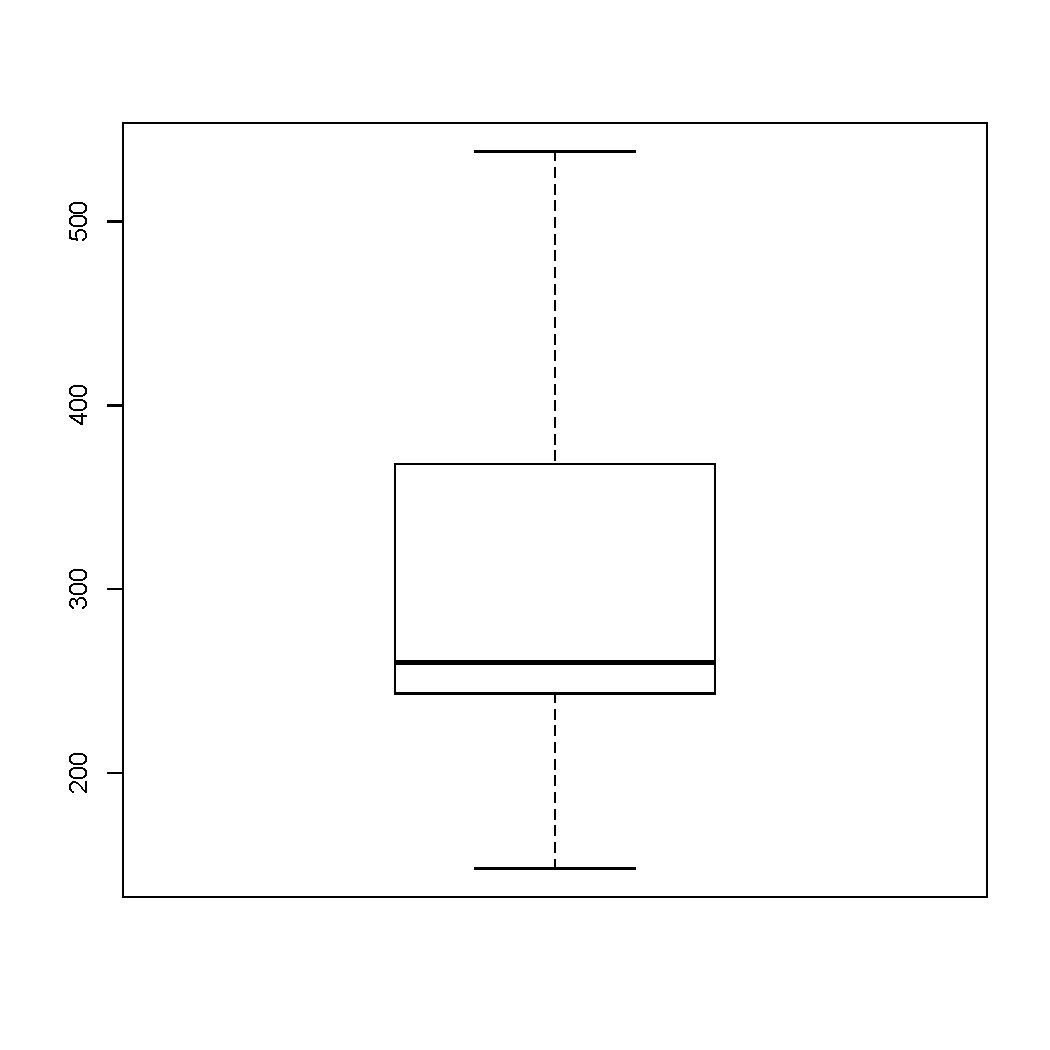
\includegraphics[scale=0.5]{sloc-boxplot.pdf}
\vspace{-1.5cm}
\end{center}
\caption{SLOC distribution among services implementations}
\label{fig:sloc-boxplot}
\end{figure}










\subsection{\textit{Framework}}
\vspace{-6mm}


As shown in Figure~\ref{fig:programGenerator}, the implementation of \neoidl{}
consists of a core (split into several Haskell modules) and 
several plugins, one for each target language (such as Swagger,
Python, or Java). The core module includes a tiny application that loads 
plugins definition and processes the program arguments, which 
specify the input \neoidl{} file, the output directory, and the languages that should be generated code from the 
input file. Moreover, the core module contains a
parser and a type checker for \neoidl{} specifications. 
We have developed the parser for \neoidl{} using \bnfc~\cite{ranta-bnfc:2012}, 
an easy to use parser generator that takes as
input a syntax specification and generates code (both abstract syntax and
parser) for different languages, including Haskell. Figure~\ref{fig:neoidl-architecture}
represents an architectural abstraction of \neoidl{} program
generator. 

\begin{figure}[b]
\begin{center}
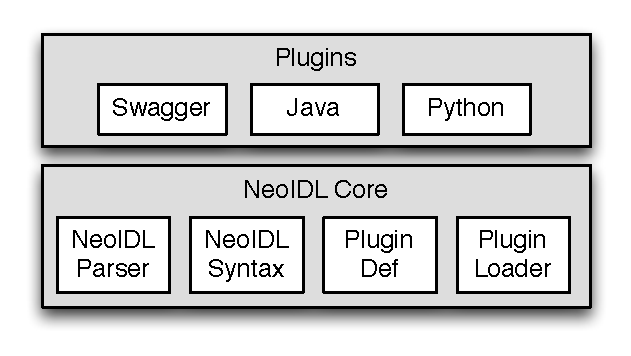
\includegraphics[scale=0.6]{neoidl.pdf}
\vspace{-.5cm}
\end{center}
\caption{Major architectural components of \neoidl{} program generator.}
\label{fig:neoidl-architecture} 
\end{figure}

In the remaining of this section
we present details about the implementation of two
\neoidl{} Haskell modules: 
\texttt{PluginDef} and \texttt{PluginLoader}. The first states the
organization of a \neoidl{} plugin and the second is responsible for
loading all available plugins. The details here are
particularly useful for those who want to develop extensible architectures
using Haskell. 


\subsubsection{PluginDef component}{\label{sec:plugindef}}

\neoidl{} plugins must comply 
with a few design rules that \texttt{PluginDef}
states. \texttt{PluginDef} is a Haskell module that 
declares two data types (\texttt{Plugin} and
\texttt{GeneratedFile}) and a type signature
(\texttt{Transform = Module -> [GeneratedFile]}) 
defining a family of functions that map a \neoidl{} module into 
a list of files whose contents are the results of the 
transformation process.

According to these design rules, each \neoidl{} plugin must declare an instance of the
\texttt{Plugin} data type and implement functions according to the
\texttt{Transform} type signature. Moreover, the 
\texttt{Plugin} instance must be named as \texttt{plugin}, so that the
\texttt{PluginLoader} component will be able to obtain the necessary 
data for executing a given plugin. Indeed, the execution of a plugin
consists of applying the respective \texttt{transformation} function for a
\neoidl{} module, producing as result a list of files that consists of 
a name and a \texttt{Doc} as file content.\footnote{The \texttt{Doc} data type
comes from the John Hughes Pretty Printer library.}  

As an alternative, we could have implemented a Haskell type class~\cite{jones-typeClasses:1995} 
exposing operations for obtaining the necessary data for a given
plugin. Although this approach might seem more natural for specifying
design rules for a pluggable architecture in Haskell, in the end it
would lead to a cumbersome approach to our problem. The main reason
for discarding this alternative approach was the need to (a) implement 
a data type, (b) make this data type an instance of the mentioned type
class, and (c) create an instance of that data type. All those steps
would be necessary for each plugin. Using our approach, the obligation
of a plugin developer is just to provide an instance of the
\texttt{Plugin} datatype, taking into account the name convention we
mentioned above. 
The \texttt{language} attribute of the \texttt{Plugin} datatype
is used for UI purpose only, so that the users will be able to obtain the list of available
plugins and select which plugins will be used during a program generation.  

% \begin{figure}[htb]
% \begin{hscode}\SaveRestoreHook 
% \column{B}{@{}>{\hspre}l<{\hspost}@{}}\column{3}{@{}>{\hspre}l<{\hspost}@{}}\column{9}{@{}>{\hspre}l<{\hspost}@{}}\column{16}{@{}>{\hspre}l<{\hspost}@{}}\column{E}{@{}>{\hspre}l<{\hspost}@{}}\>[B]{}\mathbf{module}\;\Conid{PluginDef}\;\mathbf{where}{}\<[E]\\[\blanklineskip]\>[B]{}\mathbf{data}\;\Conid{Plugin}\mathrel{=}\Conid{Plugin}\;\{\mskip1.5mu {}\<[E]\\
% \>[B]{}\hsindent{3}{}\<[3]\>[3]{}\Varid{language}{}\<[16]\>[16]{}\mathbin{::}\Conid{String},{}\<[E]\\
% \>[B]{}\hsindent{3}{}\<[3]\>[3]{}\Varid{transformation}\mathbin{::}\Conid{Transformation}{}\<[E]\\
% \>[B]{}\mskip1.5mu\}{}\<[E]\\[\blanklineskip]\>[B]{}\mathbf{data}\;\Conid{GeneratedFile}\mathrel{=}\Conid{GeneratedFile}\;\{\mskip1.5mu {}\<[E]\\
% \>[B]{}\hsindent{3}{}\<[3]\>[3]{}\Varid{name}{}\<[9]\>[9]{}\mathbin{::}\Conid{String},{}\<[E]\\
% \>[B]{}\hsindent{3}{}\<[3]\>[3]{}\Varid{content}\mathbin{::}\Conid{Doc}{}\<[E]\\
% \>[B]{}\mskip1.5mu\}{}\<[E]\\[\blanklineskip]\>[B]{}\mathbf{type}\;\Conid{Transformation}\mathrel{=}\Conid{Module}\to [\mskip1.5mu \Conid{GeneratedFile}\mskip1.5mu]{}\<[E]\ColumnHook
% \end{hscode}\resethooks
% \caption{\texttt{PluginDef} component.}
% \label{fig:plugindef}
% \end{figure}

\subsubsection{PluginLoader component}

Based on the design rules discussed in the previous section, 
the \texttt{PluginLoader} component is able to dynamically 
load the available \neoidl{} plugins. This is a Haskell
module (see Figure~\ref{lst:loader}) that exposes the
\texttt{loadPlugins} function, which returns a list  with all
available plugins. This list is obtained by compiling the Haskell plugin modules 
during the program execution and dynamically evaluating an 
expression that yields a list of \texttt{Plugin} datatype instances. 

% \begin{figure}[htb]
% \begin{hscode}\SaveRestoreHook
% \column{B}{@{}>{\hspre}l<{\hspost}@{}}\column{3}{@{}>{\hspre}l<{\hspost}@{}}\column{4}{@{}>{\hspre}l<{\hspost}@{}}\column{5}{@{}>{\hspre}l<{\hspost}@{}}\column{6}{@{}>{\hspre}l<{\hspost}@{}}\column{7}{@{}>{\hspre}l<{\hspost}@{}}\column{8}{@{}>{\hspre}l<{\hspost}@{}}\column{16}{@{}>{\hspre}l<{\hspost}@{}}\column{26}{@{}>{\hspre}l<{\hspost}@{}}\column{E}{@{}>{\hspre}l<{\hspost}@{}}\>[B]{}\mathbf{module}\;\Conid{PluginLoader}\;(\Varid{loadPlugins})\;\mathbf{where}{}\<[E]\\[\blanklineskip]\>[B]{}\mathbf{type}\;\Conid{HSFile}\mathrel{=}\Conid{String}{}\<[E]\\[\blanklineskip]\>[B]{}\Varid{dir}\mathbin{::}\Conid{String}{}\<[E]\\
% \>[B]{}\Varid{dir}\mathrel{=}\text{\tt \char34 Plugins\char34}{}\<[E]\\[\blanklineskip]\>[B]{}\Varid{loadPlugins}\mathbin{::}\Conid{IO}\;[\mskip1.5mu \Conid{Plugin}\mskip1.5mu]{}\<[E]\\
% \>[B]{}\Varid{loadPlugins}\mathrel{=}{}\<[E]\\
% \>[B]{}\hsindent{3}{}\<[3]\>[3]{}\mathbf{let}{}\<[E]\\
% \>[3]{}\hsindent{1}{}\<[4]\>[4]{}\Varid{pattern}\mathrel{=}\Varid{isSuffixOf}\;{}\<[26]\>[26]{}\text{\tt \char34 hs\char34}{}\<[E]\\
% \>[3]{}\hsindent{1}{}\<[4]\>[4]{}\Varid{path}\;\Varid{file}\mathrel{=}\Varid{dir}\mathbin{</>}\Varid{file}{}\<[E]\\
% \>[B]{}\hsindent{3}{}\<[3]\>[3]{}\mathbf{in}\;(\Varid{list}\;\Varid{dir})\bind (\Varid{compile}\mathbin{\circ}\Varid{map}\;\Varid{path}\mathbin{\circ}\Varid{filter}\;\Varid{pattern}){}\<[E]\\[\blanklineskip]\>[B]{}\Varid{dfm}\mathrel{=}\Varid{defaultFatalMessager}{}\<[E]\\
% \>[B]{}\Varid{flushOut}\mathrel{=}\Varid{defaultFlushOut}{}\<[E]\\[\blanklineskip]\>[B]{}\Varid{compile}\mathbin{::}[\mskip1.5mu \Conid{HSFile}\mskip1.5mu]\to \Conid{IO}\;[\mskip1.5mu \Conid{Plugin}\mskip1.5mu]{}\<[E]\\
% \>[B]{}\Varid{compile}\;\Varid{modules}\mathrel{=}{}\<[E]\\
% \>[B]{}\hsindent{3}{}\<[3]\>[3]{}\Varid{defaultErrorHandler}\;\Varid{dfm}\;\Varid{flushOut}\mathbin{\$}\mathbf{do}{}\<[E]\\
% \>[3]{}\hsindent{3}{}\<[6]\>[6]{}\Varid{result}\leftarrow \Varid{runGhc}\;(\Conid{Just}\;\Varid{libdir})\mathbin{\$}\mathbf{do}{}\<[E]\\
% \>[6]{}\hsindent{2}{}\<[8]\>[8]{}\mathbf{let}\;\Varid{hsModules}\mathrel{=}\Varid{map}\;\Varid{haskellModule}\;\Varid{modules}{}\<[E]\\
% \>[6]{}\hsindent{2}{}\<[8]\>[8]{}\mbox{\onelinecomment  five lines of (boilerplate) code are necessary to }{}\<[E]\\
% \>[6]{}\hsindent{2}{}\<[8]\>[8]{}\mbox{\onelinecomment  dynamically compile Haskell code using GHC}{}\<[E]\\
% \>[6]{}\hsindent{1}{}\<[7]\>[7]{}\mathbf{let}\;\Varid{exp}\mathrel{=}\Varid{buildExpresson}\;\Varid{hsModules}{}\<[E]\\
% \>[6]{}\hsindent{1}{}\<[7]\>[7]{}\Varid{plugins}\leftarrow \Varid{compileExpr}\;(\Varid{exp}\plus \text{\tt \char34 ::[Plugin]\char34}){}\<[E]\\
% \>[6]{}\hsindent{1}{}\<[7]\>[7]{}\Varid{return}\;\Varid{unsafeCoerce}\;\Varid{plugins}\mathbin{::}[\mskip1.5mu \Conid{Plugin}\mskip1.5mu]{}\<[E]\\
% \>[3]{}\hsindent{3}{}\<[6]\>[6]{}\Varid{return}\;\Varid{result}{}\<[E]\\[\blanklineskip]\>[B]{}\Varid{buildExpression}\mathbin{::}[\mskip1.5mu \Conid{HSModule}\mskip1.5mu]\to \Conid{String}{}\<[E]\\
% \>[B]{}\Varid{buildExpression}\;\Varid{hsms}\mathrel{=}\text{\tt \char34 [\char34}\plus \Varid{plugins}\plus \text{\tt \char34 ]\char34}{}\<[E]\\
% \>[B]{}\hsindent{3}{}\<[3]\>[3]{}\mathbf{where}{}\<[E]\\
% \>[3]{}\hsindent{2}{}\<[5]\>[5]{}\Varid{plugins}\mathrel{=}{}\<[16]\>[16]{}\Varid{concatMap}\;(\lambda \Varid{x}\to \Varid{x}\plus \text{\tt \char34 .plugin\char34})\;\Varid{hsms}{}\<[E]\\
% \>[3]{}\hsindent{2}{}\<[5]\>[5]{}\Varid{concat}\mathrel{=}\Varid{join}\;\text{\tt \char34 ,\char34}{}\<[E]\ColumnHook
% \end{hscode}\resethooks
% \caption{\texttt{PluginLoader} component.}
% \label{lst:loader}
% \end{figure}

We assume that
all Haskell modules within the top level \texttt{Plugins} directory must have a plugin
definition, according to the design rules of Section~\ref{sec:plugindef}.  
In Figure~\ref{lst:loader}, the \texttt{loadPlugins} function lists all files within the
\texttt{Plugins} directory, filters the Haskell files (files
 with the \texttt{``.hs''} extension), creates a qualified name to these
 files, and applies the \texttt{compile} function to the resulting
 list of qualified names. In the next step, the \texttt{compile}
 function uses the GHC API~\cite{ghc-api}
 for compiling the Haskell modules with plugin definitions and to
 evaluate an expression that produces a list with the available
 plugins. 

Our dynamic approach for loading plugins relies on the 
 GHC API, using a specific idiom to compile Haskell
 modules and execute expressions. Figure~\ref{lst:loader} shows that
 idiom in the definition of the \texttt{compile} function, although we omit some boilerplate code that is 
 necessary to compile Haskell modules using the GHC API. The last four lines of \texttt{compile} are specific to the program generator of \neoidl.
First, we build a string representation of a Haskell \texttt{list} comprising 
 all instances of the \texttt{Plugin} datatype, obtained from the
 different \neoidl{} plugins. Then, we evaluate this string
 representation of a plugin list using the \emph{meta-programming} ability
 of the \texttt{compileExpr} function, which is available in the GHC
 API. Thus, \texttt{compileExpr} dynamically evaluates a string representation of an
 expression, which leads to a value that could be used by other
 functions of a program. 
The call to \texttt{compileExpr}  
also checks the design rule that requires 
(a) a \texttt{plugin} definition
within all \neoidl{} plugins; and (b) that  
definition must be an instance of the \texttt{Plugin} data type. 
In the cases where a plugin (exposed as a Haskell module on the
top-level Plugins directory) does not comply with this design rule, 
a runtime error occurs. Accordingly, we use the default error 
handler of GHC API to report problems when loading a plugin. 
This is a new approach of using the GHC
API to dynamically check Haskell modules in pluggable architectures. 


As an example of design rule violation in the \neoidl{} architecture, 
if there is no \texttt{plugin} definition within a
plugin, the following error is reported at runtime:

\begin{tabbing}\tt
~\char36{}\char46{}\char47{}neoIDL\\
\tt ~neoIDL\char58{}~panic\char33{}~\char40{}the~\char39{}impossible\char39{}~happened\char41{}\\
\tt ~~\char40{}GHC~version~7\char46{}6\char46{}3~for~x86\char95{}64\char45{}darwin\char41{}\char58{}\\
\tt ~~~~Not~in~scope\char58{}~\char96{}Plugins\char46{}Python\char46{}plugin\char39{}
\end{tabbing}

In the last line of the above interactive section, 
\neoidl{} program generator reports that \texttt{plugin} is not defined within 
the Python plugin module. In a similar way, if the \texttt{plugin}
definition is available but it is not an instance of the \texttt{Plugin}
data type, a type error occurs during the execution of the \neoidl{}
program (see the reported message bellow, using a \texttt{plugin} definition
assigned to a String value). 


\begin{tabbing}\tt
~\char36{}\char46{}\char47{}neoIDL\\
\tt ~neoIDL\char58{}~panic\char33{}~\char40{}the~\char39{}impossible\char39{}~happened\char41{}\\
\tt ~\char40{}GHC~version~7\char46{}6\char46{}3~for~x86\char95{}64\char45{}darwin\char41{}\char58{}\\
\tt ~~Couldn\char39{}t~match~expected~type~\char96{}Plugin\char39{}\\
\tt ~~~with~actual~type~\char96{}\char91{}GHC\char46{}Types\char46{}Char\char93{}\char39{}
\end{tabbing}

Therefore, we are using GHC API to type check Haskell modules (note that Haskell is a statically typed language) during
the loading phase of a \neoidl{} execution. Next section presents the assessment of \neoidl{} considering different 
goals. 


\subsection{Linguagem}
\vspace{-6mm}


\neoidl{} simplifies service specifications by means of 
(a) mechanisms for modularizing and inheriting user defined data 
types, and (b) a concise syntax that is quite similar to the 
\emph{interface description languages} of Apache Thrift or CORBA. A 
\neoidl{} specification might be split into modules, where each
module contains several definitions. In essence, a \neoidl{} definition might be either a 
data type (using the \texttt{entity} construct) or a service describing
operations that might be reached by a given pair (URI, HTTP
method). Figures~\ref{lst:messagedata-neo}
and~\ref{lst:sentmessage-neo} present two \neoidl{} modules:
(i) the data-oriented \texttt{MessageData} module;
and the service-oriented \texttt{Message} module.

The \texttt{MessageData} module (Figure~\ref{lst:messagedata-neo})
declares an enumeration
(\texttt{MessageType}), which states the two valid types of
messages (a message must be either a \emph{message sent} or
a \emph{message received}); and a data type (\texttt{Message}),
which details the expected structure of a
message. We use a \emph{convention over configuration approach}, 
assuming that all attributes of a user defined data type are
mandatory, though it is possible to specify an attribute as being optional  
using the syntax \texttt{<Type> <Ident> = 0;}, as exemplified by
the \texttt{subject} field of the \texttt{Message} data type.

\begin{figure}[htb]
\begin{small}
\lstinputlisting[language=NeoIDL,firstnumber=1]{mensagemData.tex}
\vspace{-.5cm}
\end{small} 
\caption{Message data type specified in \neoidl}
\label{lst:messagedata-neo}
\end{figure}

The \texttt{Message} module of Figure~\ref{lst:sentmessage-neo}
specifies one service resource (\texttt{sentbox}). As explained,
we send requests for the methods of a given resource using a specific
path. In the example, the \texttt{sentbox} resource's
methods are available from the relative path
\texttt{/messages/sent}. This resource declares 
 two operations: one
\method{POST} method that might be used for
sending messages and one \method{GET} method 
that might be used for listing all messages
sent from a given sequential number.

Also according to our \emph{convention over configuration}
approach, we assume
that the arguments of \method{POST} and \method{PUT} operations
are sent in the 
request body, whereas arguments of \method{GET} operations are
either sent enclosed
with the request URL or enclosed with the URL path (in a similar way
as \method{DELETE} operations). We are able to change these conventions by
using specific annotations attached to an operation parameter.  In
these examples, conventions are used to reduce the size of services'
specifications. 

\begin{figure}[htb]
\begin{small}
\lstinputlisting[language=NeoIDL,firstnumber=1]{mensagem.tex}
\end{small}
\caption{Sent message service specification in \neoidl}
\label{lst:sentmessage-neo}
\end{figure}

To support language extensibility, \neoidl{}
specifications can be augmented through annotations. The main reason
for introducing annotations in \neoidl{} was the possibility to extend
the semantics of a specification without the need to change the 
concrete syntax of \neoidl. For instance, suppose that we want to 
express security policies for a service resource. A developer could 
change the concrete syntax of \neoidl{} for this purpose, defining new
language constructs for specifying the authentication method (based on
tokens or user passwords), the cryptographic algorithm used in the
resource request and response, and the role-based permissions to the
resource capabilities. However,
changing the concrete syntax to allow the specification of
unanticipated properties of a resource often breaks the code of the program
generator. 

Instead,
using annotations, developers might extend the language within \neoidl{}
specifications. Therefore, apart from the \neoidl{} definitions
discussed before, it is also possible to define new annotations that
might be attached to the fundamental constructs of \neoidl{} (i.e.
\texttt{module}, \texttt{enum}, \texttt{entity}, and
\texttt{resource}). Each annotation consists of a name, a target
element that indicates the \neoidl{} constructs the annotation 
might be attached to, and a list of properties. When transforming 
a specification, the list of annotations attached to a \neoidl{}
element is available to the plugins, which could consider the 
additional semantics during the program generation. Figure~\ref{lst:agent}
presents a \neoidl{} example that attaches an user defined
annotation (\texttt{SecurityPolicy}) to specify security policies 
on the \texttt{agent} resource. In the example, 
using the \texttt{SecurityPolicy} annotation we specify
that the operations of the \texttt{agent} resource
(i) must use a basic authentication mechanism, (ii)
the arguments and return values must be encoded using the
AES algorithm, and (iii) only authenticated users
having the \emph{admin} role are authorized to request the
resources. 

 
\begin{figure}
\begin{small}
\lstinputlisting[language=NeoIDL,firstnumber=1]{agent.tex}
\vspace{-.5cm}
\end{small}
\caption{\neoidl{} specification using annotations}
\label{lst:agent}
\end{figure}

In the next sections we present the lexical and 
syntactic structures of NeoIDL, considering 
the revision of August 23, 2015. Both sections 
were (almost) automatically generated by the BNF-Converter~\cite{forsberg-bnfc:2004} 
parser generator. 


\subsubsection{The lexical structure of NeoIDL}\label{sub:lexical}

\begin{enumerate}
  \item Identifiers

Identifiers \nonterminal{Ident} are unquoted strings beginning with a letter,
followed by any combination of letters, digits, and the characters {\tt \_ '},
reserved words excluded.

  \item Literals

String literals \nonterminal{String}\ have the form
\terminal{``}$x$\terminal{``}, where $x$ is any sequence of any characters
except \terminal{``} unless preceded by %% \text{\tt \char92{}}. 

Integer literals \nonterminal{Int}\ are nonempty sequences of digits.

Double-precision float literals \nonterminal{Double}\ have the structure
indicated by the regular expression $\nonterminal{digit}+ \mbox{{\it `.'}} 
\nonterminal{digit}+ (\mbox{{\it `e'}} \mbox{{\it `-'}}? \nonterminal{digit}+)?$ i.e.
two sequences of digits separated by a decimal point, optionally
followed by an unsigned or negative exponent.

  \item Reserved words and symbols
The set of reserved words is the set of terminals appearing in the grammar. 
Those reserved words that consist of non-letter characters are called symbols, 
and they are treated in a different way from those that are similar to identifiers. 
The lexer follows rules familiar from languages like Haskell, C, and Java, including longest match and spacing conventions.

The reserved words used in NeoIDL are the following: \\

\begin{tabular}{lll}
{\reserved{annotation}} &{\reserved{call}} &{\reserved{entity}} \\
{\reserved{enum}} &{\reserved{extends}} &{\reserved{float}} \\
{\reserved{for}} &{\reserved{import}} &{\reserved{int}} \\
{\reserved{module}} &{\reserved{path}} &{\reserved{resource}} \\
{\reserved{string}} & & \\
\end{tabular}\\
  
The symbols used in NeoIDL are the following: \\

\begin{tabular}{lll}
{\symb{\{}} &{\symb{\}}} &{\symb{;}} \\
{\symb{{$=$}}} &{\symb{.}} &{\symb{@}} \\
{\symb{(}} &{\symb{)}} &{\symb{0}} \\
{\symb{{$=$}{$=$}}} &{\symb{{$<$}{$>$}}} &{\symb{{$>$}}} \\
{\symb{{$>$}{$=$}}} &{\symb{{$<$}}} &{\symb{{$<$}{$=$}}} \\
{\symb{[}} &{\symb{]}} &{\symb{@get}} \\
{\symb{@post}} &{\symb{@put}} &{\symb{@delete}} \\
{\symb{/@require}} &{\symb{/@ensure}} &{\symb{/@invariant}} \\
{\symb{/@otherwise}} &{\symb{/**}} &{\symb{*/}} \\
{\symb{*}} &{\symb{@desc}} &{\symb{@param}} \\
{\symb{@consume}} &{\symb{,}} & \\
\end{tabular}\\

\end{enumerate}

\subsubsection{The syntactic structure of NeoIDL}\label{sub:syntactic}

Non-terminals are enclosed between $\langle$ and $\rangle$. 
The symbols  {\arrow}  (production),  {\delimit}  (union) 
and {\emptyP} (empty rule) belong to the following BNF notation.
All other symbols are terminals.\\

\begin{small}
\begin{tabular}{lll}
\label{lst:BNFnot}
{\nonterminal{Modulo}} {\arrow} {\terminal{module}} {\nonterminal{Ident}} {\terminal{\{}} \\ 
 \quad {\nonterminal{ListImport}} \\ 
 \quad {\nonterminal{MPath}} \\ 
 \quad {\nonterminal{ListEnum}} \\ 
 \quad {\nonterminal{ListEntity}} \\ 
 \quad {\nonterminal{ListResource}} \\ 
 \quad {\nonterminal{ListDecAnnotation}} \\ 
{\terminal{\}}}  \\
\end{tabular}\\

\begin{tabular}{lll}
{\nonterminal{Import}} & {\arrow}  &{\terminal{import}} {\nonterminal{NImport}} {\terminal{;}}  \\
\end{tabular}\\

\begin{tabular}{lll}
{\nonterminal{MPath}} & {\arrow}  &{\emptyP} \\
 & {\delimit}  &{\terminal{path}} {\terminal{{$=$}}} {\nonterminal{String}} {\terminal{;}}  \\
\end{tabular}\\

\begin{tabular}{lll}
{\nonterminal{NImport}} & {\arrow}  &{\nonterminal{Ident}}  \\
 & {\delimit}  &{\nonterminal{Ident}} {\terminal{.}} {\nonterminal{NImport}}  \\
\end{tabular}\\

\begin{tabular}{lll}
{\nonterminal{Entity}} & {\arrow}  &{\nonterminal{ListDefAnnotation}} {\terminal{entity}} {\nonterminal{Ident}} {\terminal{\{}} {\nonterminal{ListProperty}} {\terminal{\}}} {\terminal{;}}  \\
 & {\delimit}  &{\nonterminal{ListDefAnnotation}} {\terminal{entity}} {\nonterminal{Ident}} {\terminal{extends}} {\nonterminal{Ident}} {\terminal{\{}} {\nonterminal{ListProperty}} {\terminal{\}}} {\terminal{;}}  \\
\end{tabular}\\

\begin{tabular}{lll}
{\nonterminal{Enum}} & {\arrow}  &{\terminal{enum}} {\nonterminal{Ident}} {\terminal{\{}} {\nonterminal{ListValue}} {\terminal{\}}} {\terminal{;}}  \\
\end{tabular}\\

\begin{tabular}{lll}
{\nonterminal{DecAnnotation}} & {\arrow}  &{\terminal{annotation}} {\nonterminal{Ident}} {\terminal{for}} {\nonterminal{AnnotationType}} {\terminal{\{}} {\nonterminal{ListProperty}} {\terminal{\}}} {\terminal{;}}  \\
\end{tabular}\\

\begin{tabular}{lll}
{\nonterminal{DefAnnotation}} & {\arrow}  &{\terminal{@}} {\nonterminal{Ident}} {\terminal{(}} {\nonterminal{ListAssignment}} {\terminal{)}} {\terminal{;}}  \\
\end{tabular}\\

\begin{tabular}{lll}
{\nonterminal{Parameter}} & {\arrow}  &{\nonterminal{Type}} {\nonterminal{Ident}} {\nonterminal{Modifier}}  \\
\end{tabular}\\

\begin{tabular}{lll}
{\nonterminal{Assignment}} & {\arrow}  &{\nonterminal{Ident}} {\terminal{{$=$}}} {\nonterminal{Value}}  \\
\end{tabular}\\

\begin{tabular}{lll}
{\nonterminal{Modifier}} & {\arrow}  &{\emptyP} \\
 & {\delimit}  &{\terminal{{$=$}}} {\terminal{0}}  \\
\end{tabular}\\

\begin{tabular}{lllllllll}
{\nonterminal{AnnotationType}} & {\arrow}  &{\terminal{resource}}  
 & {\delimit}  &{\terminal{enum}}  
 & {\delimit}  &{\terminal{entity}}  
 & {\delimit}  &{\terminal{module}} 
\end{tabular}\\

\begin{tabular}{lll}
{\nonterminal{Resource}} & {\arrow}  &{\nonterminal{ListDefAnnotation}} {\terminal{resource}} {\nonterminal{Ident}} {\terminal{\{}} {\terminal{path}} {\terminal{{$=$}}} {\nonterminal{String}} {\terminal{;}} {\nonterminal{ListCapacity}} {\terminal{\}}} {\terminal{;}}  \\
\end{tabular}\\

\begin{tabular}{lll}
{\nonterminal{Capacity}} & {\arrow}  &{\nonterminal{NeoDoc}} {\nonterminal{ListDefNAnnotation}} {\nonterminal{Method}} {\nonterminal{Type}} {\nonterminal{Ident}} {\terminal{(}} {\nonterminal{ListParameter}} {\terminal{)}} {\terminal{;}}  \\
\end{tabular}\\


\begin{tabular}{lllllllll}
{\nonterminal{Method}} & {\arrow}  &{\terminal{@get}} 
 & {\delimit}  &{\terminal{@post}} 
 & {\delimit}  &{\terminal{@put}}  
 & {\delimit}  &{\terminal{@delete}} 
\end{tabular}\\
\end{small}    











\section{Avaliação empírica}
\vspace{-6mm}

% anexar script de transcrição.

\subsection{Expressividade}
\vspace{-6mm}



In Section~\ref{sub:experience} we presented the comparison in SLOC between the contracts
specification in NeoIDL and the resultant code generated by the framework. Another
relevant issue is a comparison of expressiveness of contracts written in \neoidl{} and other popular
languages with the same purpose (specifying contracts for REST services). In this context,
we compared \neoidl{} specifications with Swagger specifications, a language that has been increasily used by the industry.
Swagger ~\cite{swagger} contracts may by written in JSON and Yaml, both based on key-value structure.

In a collaborative work with the Brazilian Army,
we obtained a portion of their contracts' specifications in Swagger (44 in total), specified with version 1.2.
Our first step was to rewrite these specifications in \neoidl{} and thus compare the total
number of lines of code (which might serve as a metric of expressiveness).
The 44 contracts in Swagger amount to 13921 lines of specification, while the same set of contracts in NeoIDL comprises 5140 lines of specification. Thus, the average reduction was about 63\%. In others words, it means that 10 lines of structured Swagger specification require
about 4 lines of \neoidl{} specification. In this analysis we only considered \emph{physical lines of code}, ignoring 
blank lines and lines consisting of delimiters only. The Appendix A shows a sample contract we analised.

The reduction in number of lines is not the same in all contracts. For instance, a given service\footnote{For confidentiality reasons, the real names of contracts were omitted.} required 367 lines of Swagger specification and 112 lines of \neoidl{} specification. This case  
represents a reduction of about 69\%. On the other hand, another service contract required 
81 lines of specification in Swagger and 42 lines of \neoidl{} specification. In this case, the SLOC decrease was slightly less than 50\%.

The size of the original contract has only a small influence in the observed expressiveness. 
Therefore, we cannot assume that \emph{the bigger the contract is in Swagger 
the bigger is the improvement (with respect to the smaller specification size) of \neoidl}. We 
also realized that the use of a more descritive documentation, the number of entities, and the number of capacities do not correlate to the advantageous reduction of lines of code during a 
transformation of Swagger specifications into \neoidl{} specifications. Therefore, it seems that 
the benefits do not relate to the size of the original specifications.  
Table~\ref{tab:size-corr} presents the correlation between the improvement of 
expressiveness (measured as the percentage of reduction obtained 
after transforming Swagger specifications into \neoidl{} specifications) and 
some metrics related to the size of the original Swagger specifications.

\begin{table}[htb]
\caption{Correlation of the Expressiveness Improvement with the size of the Swagger specifications}
\begin{center}
\begin{tabular}{lrr} 
\toprule
Metric & Pearson's correlation & \emph{p-value} \\ \hline \hline 
LOC of Swagger specification & 0.19 &  0.20 \\ 
Number of services & 0.14 & 0.35 \\ 
Number of capacities & 0.14 & 0.34 \\
Number of entities & 0.20 & 0.18 \\ \bottomrule 
\end{tabular} 
\end{center}
\label{tab:size-corr}
\end{table}





\subsection{Potencial de reuso}



Similar to \neoidl{}, Swagger presents 
some mechanisms to reuse user defined structures. Nevertheless, 
this feature is almost ignored in the set of contracts we analysed, which 
leads to the duplication of entities' definition across different 
Swagger specifications. This might have occurred either due to the 
nonintuitive construct for reusing definitions in Swagger (based on 
references to JSON files) and the difficulties to identify 
that one entity had already been specified in another contract.
After analysing the 44 Swagger specifications, we realized that 40 entities 
have been specified in  more than one contract. Actually, one specific 
entity is present in 12 distinct Swagger contracts. 




 
\section{Extensão da NeoIDL para \designbycontract{}}

Influência de Eiffel, JML e Spec\#

Eiffel assertions are Boolean expressions, with a few extensions such as the old
notation. Since the whole power of Boolean expressions is available, they may
include function calls. Because the full power of the language is available to
write these functions, the conditions they express can be quite sophisticated.
\cite{meyer1992applying}

 
 
\subsection{Proposta: Serviços com Desing-by-Contract}
\vspace{-6mm}

Os benefícios esperados pela adoção da arquitetura orientada a serviços
somente serão auferidos com a concepção adequada de cada serviço. 
Por essa razão, é necessário planejar o projeto dos serviços criteriosamente
antes de lançar mão do desenvolvimento, com preocupação especial em garantir
um nível aceitável de estabilidade aos consumidores de cada serviço.
Nessa etapa do projeto de desenho da solução, a especificação do contrato do
serviço (Web API) exerce uma função fundamental. 

Na sociedade civil, contratos são meios de se formalizar acordo entre partes a
fim de definir os direitos e deveres de cada parte e buscar atingir o
objetivo esperado dentro de determinadas regras. Cada parte espera que as outras
cumpram com suas obrigações.
Por outro lado, sabe-se que o descumprimeto das obrigações costuma implicar de
penalizações até o desfazimento do contrato. 

Contratos entre serviços Web seguem em uma linha análoga. O desenho das
capacidades (operações) e dos dados das mensagens correspondem aos
termos do contrato no sentido do que o consumidor deve esperar do serviço
provedor. Porém identificou-se, após ampla pesquisa realizada sobre o tema, que
as linguagens disponíves para especificação de contratos atingem apenas esse
nível de garantias. No contexto de webservices em REST, conforme descrito na
seção \ref{secaoREST}, há ainda a ausência de padrão para especificação
contratos, tal como ocorre com o WSDL adotado em SOAP.

A proposta deste trabalho é extender os níveis de garantias, de modo a promover
um patamar adicional com obrigações mutuas entre os serviços (consumidor e
provedor). Isso se dá para adoção do conceito de Design-by-Contract (debatido
na seção \ref{Design-by-Contract}) em que a execução da
capacidade do serviço garantirá a execução, desde que satisfeitas as condições
prévias. O detalhamento do processo é exposto nas seções que se seguem.

\vspace{-6mm}

\subsubsection{Modelo de operação}
\vspace{-6mm}

As garantias para execução dos serviços são estabelecidas em duas etapas: pré- e
pós-condições. Nas pré-condições o provedor do serviço estabelece os requisitos
para que o serviço possa ser executado. A etapa de pós-condições tem o papel de
validar se a mensagem de retorno do serviço possui resultados válidos.

O diagrama da Figura \ref{FigServiceDbC} descreve como ocorre a operação das
pré- e pós-condições. O processo se inicia com a chamada à capacidade do serviço e a
identificação da existência de uma pré-condição. Caso tenham sido estabelecidas 
pré-condições, essas são avaliadas. Caso alguma delas não tenham sido
satisfeitas, o serviço principal não é processado e o provedor do serviço
retornar o código de falha definido no contrato correspondente.


\begin{figure}[!htb]
\centering
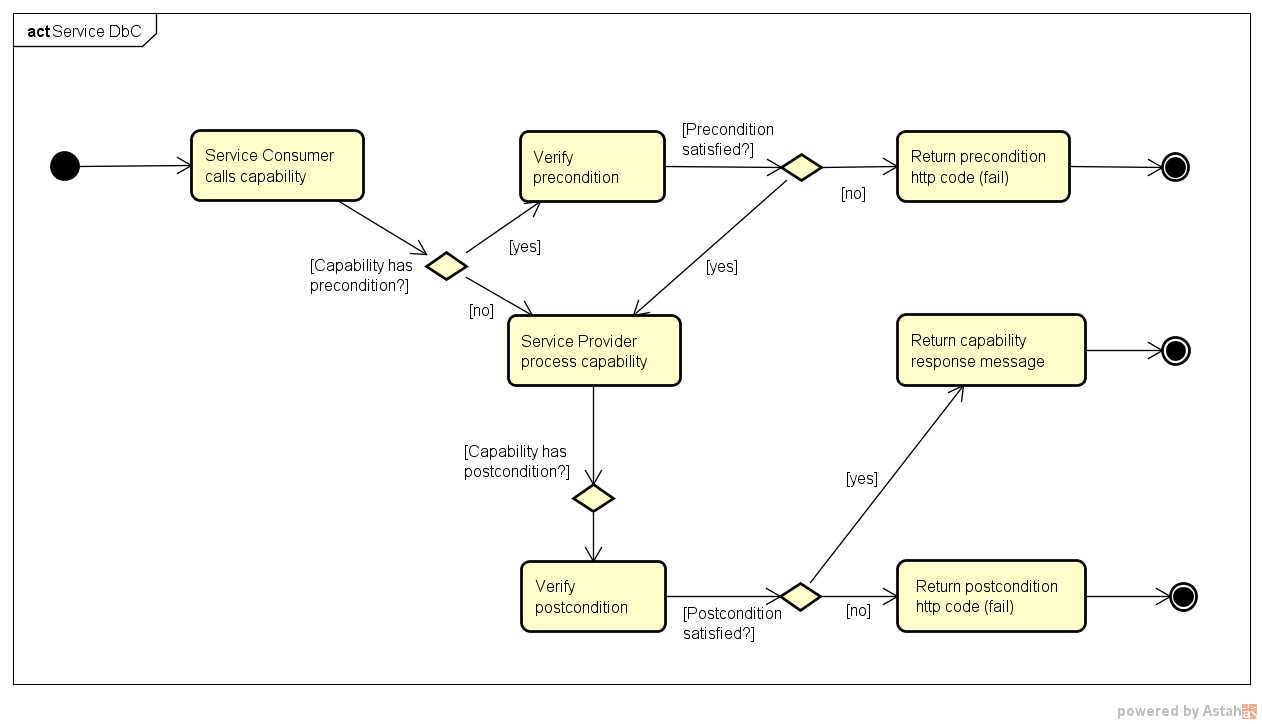
\includegraphics[width=\textwidth,trim = 0mm 5mm 0mm 0mm,clip]{ServiceDbC.png}
\caption{Digrama de atividades com verificação de pré e pós condições}
\label{FigServiceDbC}
\end{figure}

Caso tenham sido definidas pós-condições, essas são acionadas após o
processamento da capacidade, porém antes do retorno ao consumidor do serviço.
Assim, conforme Figura \ref{FigServiceDbC}, visando não entregar ao cliente uma
mensagem ou situação incoerente, as pós-condições são validadas. Caso todas as
pós-condições tenham sido satisfeitas, a mensagem de retorno é encaminhada ao
cliente. Caso contrário, será retornado o código de falha.


\vspace{-6mm}


\subsubsection{Verificação das pré-condições}
\vspace{-6mm}

As pré-condições podem ser do tipo baseado nos parâmetros da requisição ou do
tipo baseado na chamada a outro serviço. Denominamos, para o contexto desta
dissertação, de básica a pré-condição baseada apenas nos parâmetros da
requisição (atributos da chamada ao serviço). Nessa validação é direta,
comparando os valores passados com os valores admitidos. 

No caso das pré-condições baseadas em serviços, é realizada chamada a outro
serviço para verificar se uma determinada condição é satisfeita. Este modo de
funcionamento, que se assemelha a uma composição de serviço, é mais versátil, pois permite
validações de condições complexas sem que a lógica associada seja conhecida pelo
cliente. Assim, os contratos que estabelecem esse tipo de
pré-condição se mantem simples.

A Figura \ref{FigServicePrecondition} detalha as etapas de verificação de cada
pré-condição. Nota-se que a saída para as situações de desatendimento às
pré-condições, independentemente do tipo, é o mesmo. O objetivo desta abordagem
é simplificar o tratametno de exceção no consumidor.

\begin{figure}[!htb]
\centering
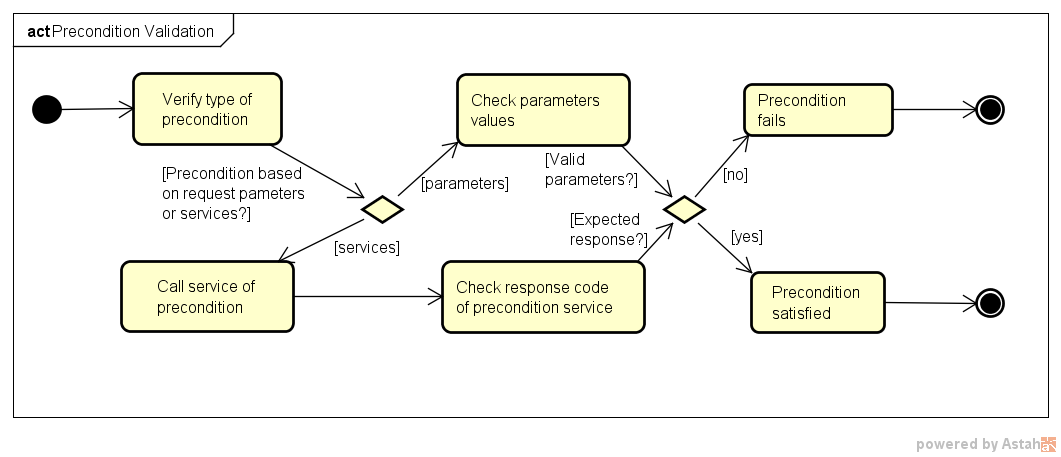
\includegraphics[width=\textwidth,trim = 0mm 5mm 0mm 0mm,clip]{PreconditionValidation.png}
\caption{Diagrama de atividades do processamento da pré-condição}
\label{FigServicePrecondition}
\end{figure}


\subsubsection{Verificação das pós-condições}
\vspace{-6mm}

\begin{figure}[!htb]
\centering
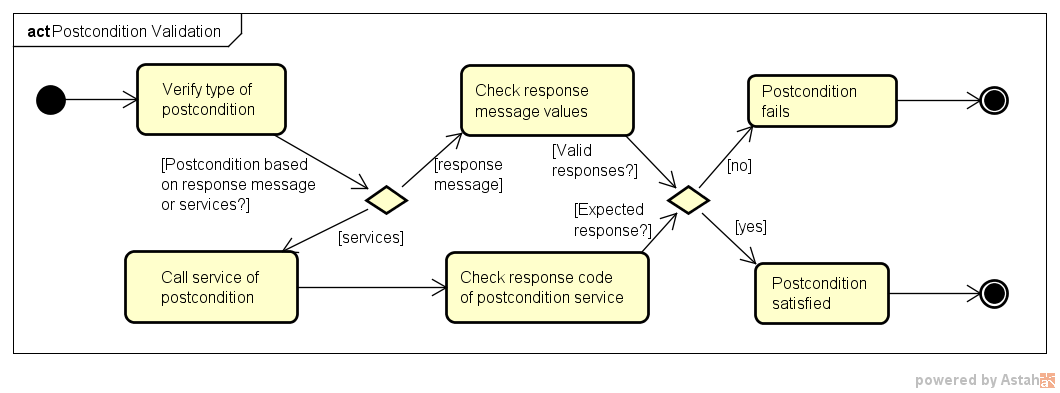
\includegraphics[width=\textwidth,trim = 0mm 5mm 0mm
0mm,clip]{PostconditionValidation.png} 
\vspace{-6mm}
\caption{Diagrama de atividades do processamento da pós-condição}
\label{FigServicePostcondition}
\end{figure}

A verificação das pós-condições acontece de modo muito similar a das
pré-condições. Há também os dois tipos, baseado em valores e em chamadas a
outros serviços. O diferencial está em que a validação dos valores passa a
ocorrer a partir dos valores contidos na mensagem de retorno. A Figura
\ref{FigServicePostcondition} descreve as etapas necessárias para validação de
cada pré-condição.

	
	
	
	

\subsection{Extensão da linguagem}

\subsubsection{Precondição básica}

\begin{figure}[htb]
\begin{small}
\lstinputlisting[language=NeoIDL,firstnumber=1]{DBCsimple.neo}
\end{small}
\caption{Exemplo da notação DBC básica na \neoidl{}}
\label{lst:DBCService}
\end{figure} 

\subsubsection{Pós-condição básica}

\ldots



\subsubsection{Precondição com chamada a serviço}

\begin{figure}[htb]
\begin{small}
\lstinputlisting[language=NeoIDL,firstnumber=1]{DBCservice.neo}
\end{small}
\caption{Exemplo da notação DBC na \neoidl{} com chamada a serviço}
\label{lst:DBCService}
\end{figure} 


\subsubsection{Pós-condição com chamada a serviço}

\ldots

\subsection{Estudo de caso: plugin twisted}

\ldots

\subsubsection{Arquitetura}

% Diagrama da estrutura do código gerado


\subsubsection{Geração de código}